\documentclass[11pt,a4paper]{article}
\usepackage[margin=2.5cm]{geometry}
\usepackage{amsmath,amssymb,amsthm,tikz,xcolor,fancyvrb,hyperref}
\usepackage{fontspec}\setmonofont{DejaVu Sans Mono}[Scale=0.72]
\newtheorem{theorem}{Slopollary}\setcounter{theorem}{1}
\theoremstyle{remark}\newtheorem*{remark}{Remarks}
\title{\textbf{Slopollary 2}\\[2pt]\large Every zeta zero picks a point on the Mandelbrot set's main cardioid}
\author{Maths Slop (@slopollary)}
\date{25 November 2026}
\begin{document}\maketitle

\begin{abstract}
The Riemann hypothesis is now a theorem (Alp\"oge, 20 November 2026, formally
verified in Lean). We record a consequence linking two famous pictures: each
nontrivial zero $\rho$ of $\zeta$ determines a quadratic map $z\mapsto z^{2}+c_\rho$
whose parameter $c_\rho$ lies exactly on the boundary of the main cardioid of the
Mandelbrot set. As the zeros climb the critical line, the parameters march into
the cusp at $\tfrac14$.
\end{abstract}

\section*{Statement}
For a nontrivial zero $\rho$ of the Riemann zeta function put
\[
  \mu_\rho = 1-\frac1\rho ,\qquad c_\rho=\frac14\Bigl(1-\frac1{\rho^{2}}\Bigr).
\]
Recall that the boundary of the main cardioid of the Mandelbrot set is the curve
$\bigl\{\tfrac{\mu}{2}-\tfrac{\mu^{2}}{4} : |\mu|=1\bigr\}$; these are exactly the
parameters $c$ for which $z\mapsto z^{2}+c$ has a fixed point with multiplier $\mu$
of modulus one (a \emph{neutral} fixed point).

\begin{theorem}
For every nontrivial zero $\rho$ of $\zeta$:
\begin{enumerate}
  \item $|\mu_\rho|=1$ and $c_\rho=\tfrac{\mu_\rho}{2}-\tfrac{\mu_\rho^{2}}{4}$, so
        $c_\rho$ lies on the boundary of the main cardioid of the Mandelbrot set;
  \item equivalently, $z\mapsto z^{2}+c_\rho$ has the neutral fixed point
        $z_0=\mu_\rho/2$: it satisfies $z_0^{2}+c_\rho=z_0$ and $|2z_0|=1$.
\end{enumerate}
\end{theorem}

\begin{proof}
The identity $\tfrac14(1-\rho^{-2})=\tfrac{\mu}{2}-\tfrac{\mu^{2}}{4}$ with
$\mu=1-\rho^{-1}$ holds for every $\rho\neq0$, since
$\tfrac14-\bigl(\tfrac{\mu}{2}-\tfrac{\mu^{2}}{4}\bigr)=\tfrac14(1-\mu)^{2}=\tfrac1{4\rho^{2}}$.
By the Riemann hypothesis $\operatorname{Re}\rho=\tfrac12$, so $\rho$ is equidistant
from $0$ and $1$, and $|\mu_\rho|=|\rho-1|/|\rho|=1$. For (2),
$z_0^{2}+c_\rho=\tfrac{\mu^{2}}{4}+\tfrac{\mu}{2}-\tfrac{\mu^{2}}{4}=z_0$ and $2z_0=\mu_\rho$.
\end{proof}

\begin{center}
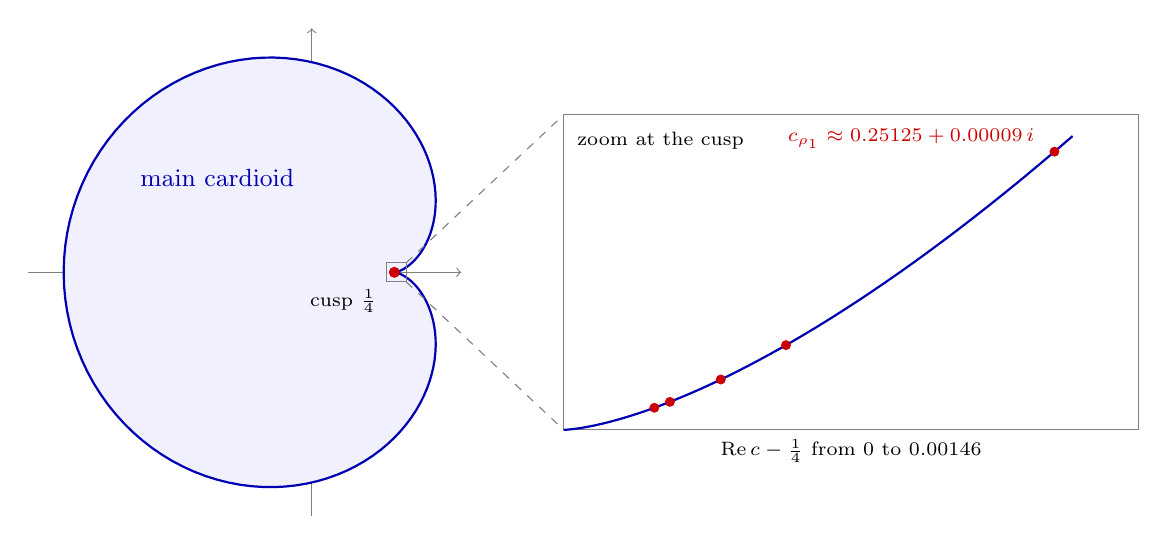
\begin{tikzpicture}
\begin{scope}
  \draw[->,gray] (-3.6,0)--(1.9,0);
  \draw[->,gray] (0,-3.1)--(0,3.1);
  \draw[thick,blue!70!black,fill=blue!6] (1.0500,0.0000) -- (1.0516,0.0001) -- (1.0565,0.0005) -- (1.0645,0.0017) -- (1.0755,0.0040) -- (1.0896,0.0079) -- (1.1064,0.0135) -- (1.1259,0.0214) -- (1.1478,0.0318) -- (1.1718,0.0449) -- (1.1977,0.0612) -- (1.2252,0.0808) -- (1.2539,0.1039) -- (1.2836,0.1308) -- (1.3139,0.1617) -- (1.3443,0.1966) -- (1.3745,0.2357) -- (1.4040,0.2791) -- (1.4326,0.3268) -- (1.4597,0.3787) -- (1.4849,0.4349) -- (1.5079,0.4953) -- (1.5281,0.5598) -- (1.5452,0.6282) -- (1.5588,0.7003) -- (1.5685,0.7760) -- (1.5739,0.8550) -- (1.5747,0.9370) -- (1.5706,1.0216) -- (1.5611,1.1087) -- (1.5461,1.1977) -- (1.5253,1.2883) -- (1.4984,1.3800) -- (1.4653,1.4725) -- (1.4258,1.5653) -- (1.3798,1.6578) -- (1.3271,1.7497) -- (1.2678,1.8403) -- (1.2018,1.9293) -- (1.1292,2.0160) -- (1.0500,2.1000) -- (0.9643,2.1808) -- (0.8723,2.2578) -- (0.7742,2.3306) -- (0.6701,2.3986) -- (0.5604,2.4615) -- (0.4453,2.5187) -- (0.3252,2.5698) -- (0.2005,2.6144) -- (0.0716,2.6521) -- (-0.0612,2.6826) -- (-0.1973,2.7055) -- (-0.3362,2.7206) -- (-0.4775,2.7275) -- (-0.6206,2.7261) -- (-0.7649,2.7162) -- (-0.9099,2.6975) -- (-1.0550,2.6702) -- (-1.1996,2.6339) -- (-1.3431,2.5888) -- (-1.4849,2.5349) -- (-1.6245,2.4722) -- (-1.7611,2.4009) -- (-1.8943,2.3211) -- (-2.0234,2.2330) -- (-2.1479,2.1368) -- (-2.2672,2.0328) -- (-2.3809,1.9214) -- (-2.4883,1.8028) -- (-2.5890,1.6776) -- (-2.6826,1.5461) -- (-2.7686,1.4088) -- (-2.8467,1.2661) -- (-2.9164,1.1186) -- (-2.9775,0.9669) -- (-3.0297,0.8115) -- (-3.0728,0.6530) -- (-3.1064,0.4919) -- (-3.1306,0.3290) -- (-3.1451,0.1648) -- (-3.1500,0.0000) -- (-3.1451,-0.1648) -- (-3.1306,-0.3290) -- (-3.1064,-0.4919) -- (-3.0728,-0.6530) -- (-3.0297,-0.8115) -- (-2.9775,-0.9669) -- (-2.9164,-1.1186) -- (-2.8467,-1.2661) -- (-2.7686,-1.4088) -- (-2.6826,-1.5461) -- (-2.5890,-1.6776) -- (-2.4883,-1.8028) -- (-2.3809,-1.9214) -- (-2.2672,-2.0328) -- (-2.1479,-2.1368) -- (-2.0234,-2.2330) -- (-1.8943,-2.3211) -- (-1.7611,-2.4009) -- (-1.6245,-2.4722) -- (-1.4849,-2.5349) -- (-1.3431,-2.5888) -- (-1.1996,-2.6339) -- (-1.0550,-2.6702) -- (-0.9099,-2.6975) -- (-0.7649,-2.7162) -- (-0.6206,-2.7261) -- (-0.4775,-2.7275) -- (-0.3362,-2.7206) -- (-0.1973,-2.7055) -- (-0.0612,-2.6826) -- (0.0716,-2.6521) -- (0.2005,-2.6144) -- (0.3252,-2.5698) -- (0.4453,-2.5187) -- (0.5604,-2.4615) -- (0.6701,-2.3986) -- (0.7742,-2.3306) -- (0.8723,-2.2578) -- (0.9643,-2.1808) -- (1.0500,-2.1000) -- (1.1292,-2.0160) -- (1.2018,-1.9293) -- (1.2678,-1.8403) -- (1.3271,-1.7497) -- (1.3798,-1.6578) -- (1.4258,-1.5653) -- (1.4653,-1.4725) -- (1.4984,-1.3800) -- (1.5253,-1.2883) -- (1.5461,-1.1977) -- (1.5611,-1.1087) -- (1.5706,-1.0216) -- (1.5747,-0.9370) -- (1.5739,-0.8550) -- (1.5685,-0.7760) -- (1.5588,-0.7003) -- (1.5452,-0.6282) -- (1.5281,-0.5598) -- (1.5079,-0.4953) -- (1.4849,-0.4349) -- (1.4597,-0.3787) -- (1.4326,-0.3268) -- (1.4040,-0.2791) -- (1.3745,-0.2357) -- (1.3443,-0.1966) -- (1.3139,-0.1617) -- (1.2836,-0.1308) -- (1.2539,-0.1039) -- (1.2252,-0.0808) -- (1.1977,-0.0612) -- (1.1718,-0.0449) -- (1.1478,-0.0318) -- (1.1259,-0.0214) -- (1.1064,-0.0135) -- (1.0896,-0.0079) -- (1.0755,-0.0040) -- (1.0645,-0.0017) -- (1.0565,-0.0005) -- (1.0516,-0.0001) -- (1.0500,0.0000) -- cycle;
  \fill[red!80!black] (1.05,0) circle (2pt);
  \node[anchor=north east] at (0.95,-0.1) {\scriptsize cusp $\tfrac14$};
  \node[blue!70!black] at (-1.2,1.2) {\small main cardioid};
  \draw[gray] (0.95,-0.12) rectangle (1.2,0.12);
  \draw[gray,dashed] (1.2,0.12)--(3.2,2.0);
  \draw[gray,dashed] (1.2,-0.12)--(3.2,-2.0);
\end{scope}
\begin{scope}[shift={(3.2,-2.0)}]
  \draw[gray] (0,0) rectangle (7.3,4.0);
  \draw[thick,blue!70!black] (0.0000,0.0000) -- (0.0019,0.0000) -- (0.0077,0.0002) -- (0.0173,0.0005) -- (0.0308,0.0012) -- (0.0482,0.0024) -- (0.0694,0.0041) -- (0.0944,0.0066) -- (0.1233,0.0098) -- (0.1561,0.0140) -- (0.1927,0.0191) -- (0.2332,0.0255) -- (0.2775,0.0331) -- (0.3256,0.0421) -- (0.3777,0.0525) -- (0.4335,0.0646) -- (0.4932,0.0784) -- (0.5568,0.0940) -- (0.6242,0.1116) -- (0.6955,0.1313) -- (0.7706,0.1531) -- (0.8495,0.1773) -- (0.9323,0.2038) -- (1.0190,0.2329) -- (1.1095,0.2646) -- (1.2038,0.2990) -- (1.3020,0.3364) -- (1.4040,0.3767) -- (1.5098,0.4201) -- (1.6195,0.4667) -- (1.7330,0.5167) -- (1.8504,0.5701) -- (1.9716,0.6270) -- (2.0966,0.6877) -- (2.2255,0.7521) -- (2.3582,0.8204) -- (2.4947,0.8927) -- (2.6350,0.9692) -- (2.7792,1.0498) -- (2.9272,1.1349) -- (3.0790,1.2244) -- (3.2347,1.3185) -- (3.3941,1.4173) -- (3.5574,1.5209) -- (3.7245,1.6295) -- (3.8954,1.7431) -- (4.0701,1.8618) -- (4.2487,1.9858) -- (4.4310,2.1152) -- (4.6171,2.2501) -- (4.8071,2.3906) -- (5.0009,2.5368) -- (5.1984,2.6889) -- (5.3998,2.8469) -- (5.6049,3.0110) -- (5.8138,3.1812) -- (6.0266,3.3578) -- (6.2431,3.5408) -- (6.4634,3.7302);
  \fill[red!80!black] (6.2331,3.5323) circle (1.8pt);
  \fill[red!80!black] (2.8237,1.0752) circle (1.8pt);
  \fill[red!80!black] (1.9959,0.6387) circle (1.8pt);
  \fill[red!80!black] (1.3493,0.3549) circle (1.8pt);
  \fill[red!80!black] (1.1516,0.2798) circle (1.8pt);
  \node[red!80!black,anchor=south east] at (6.1,3.45) {\scriptsize $c_{\rho_1}\approx 0.25125+0.00009\,i$};
  \node[anchor=north west] at (0.05,3.9) {\scriptsize zoom at the cusp};
  \node[anchor=north] at (3.65,0) {\scriptsize $\operatorname{Re}c-\tfrac14$ from $0$ to $0.00146$};
\end{scope}
\end{tikzpicture}

\small Left: the main cardioid. Right: a zoom at the cusp (height $10^{-4}$, not to scale)
showing $c_\rho$ for the first five zeros, approaching $\tfrac14$ from the right.
\end{center}

\begin{remark}
(i) \emph{What is classical.} That $|1-1/\rho|=1$ on the critical line is the
fact behind Li's criterion, and the cardioid parametrisation is standard. What we
could not find stated is the composition: the zeta zeros index points of the
Mandelbrot cardioid. The closest work we know is Kawahira (arXiv:1602.06843), who
shows that RH with simple zeros is equivalent to every nontrivial zero being an
indifferent fixed point of $\nu(z)=z-\zeta(z)/(z\zeta'(z))$; the multiplier there is
also $1-1/\rho$, but no quadratic family or Mandelbrot set appears.

(ii) \emph{Rotation angle.} For $\rho=\tfrac12+i\gamma$ one has
$\mu_\rho=e^{i\theta}$ with $\theta=2\arctan\frac{1}{2\gamma}$, the angle under which
$\rho$ sees the segment $[0,1]$. As $\gamma\to\infty$, $\theta\to0$ and $c_\rho\to\tfrac14$.

(iii) \emph{Converse.} If $\rho\neq0$, $\operatorname{Re}\rho\neq-\tfrac12$ and
$c_\rho$ lies on the cardioid, then $\operatorname{Re}\rho=\tfrac12$ (formalised
below). Since nontrivial zeros have $0<\operatorname{Re}\rho<1$, the statement
``every $c_\rho$ lies on the main cardioid'' is equivalent to the Riemann
hypothesis; that last step uses the critical strip and is not formalised.

(iv) \emph{Relation to Slopollary 1.} $1-4c_\rho=1/\rho^{2}$ lies on the cardioid
$r=2(1+\cos\varphi)$, the inversion about its focus of the parabola of Slopollary 1.
\end{remark}

\section*{Formalisation (Lean 4 + Mathlib)}
The statement is phrased against Mathlib's \texttt{RiemannHypothesis}, taken as a
hypothesis. The file below compiles without errors or warnings on
\texttt{live.lean-lang.org} (Lean 4.37.0-rc1 with current Mathlib, 25 November 2026);
\texttt{\#print axioms} reports only \texttt{propext}, \texttt{Classical.choice}
and \texttt{Quot.sound} for all three main theorems.
\VerbatimInput[frame=single,rulecolor=\color{gray!50}]{Slopollary2.lean}
\end{document}
